\chapter{Concurrency}
\label{ch:concurrency}

\section*{Required reading}

\begin{itemize}
\item \href{https://www.postgresql.org/docs/13/mvcc.html}{Concurrency control} in PostgreSQL manual.
\item \citep[Chapter 22]{connolly:2015:database} discusses concurrency in general but focuses first on locking rather than multi-version concurrency control (as PostgreSQL supports).
\item \citep{haerder:1983:principles} introduce the ACID principles.
\item You must have access to the shared database server.
\end{itemize}

\section{Situation}

\subsection{Units of work}

We will assume a transaction to be a ``bounded unit of work'' \citep{fowler:2003:patterns}.
(We have already met transaction handling as a basic ``undo'' facility on a practical level.) 
A transaction is identifed to the database by the following SQL. 

\begin{minted}{postgresql}
BEGIN; --- starts the transaction

--- statements go here
INSERT ... ;
UPDATE ... ;
DELETE ... ; --- etc

COMMIT; --- finishes the transaction, saving changes
-- or
ROLLBACK; --- finishes the transaction, discards changes
\end{minted}

We have already met the \mintinline{postgresql}{SAVEPOINT} keyword to do partial rollbacks.
For this chapter we will ignore this usage.

\subsection{Concurrent access}

Databases normally have a number of concurrent clients connected at any one time, \autoref{fig:concurrent-clients}.

\begin{figure}[htbp]
  \centering
  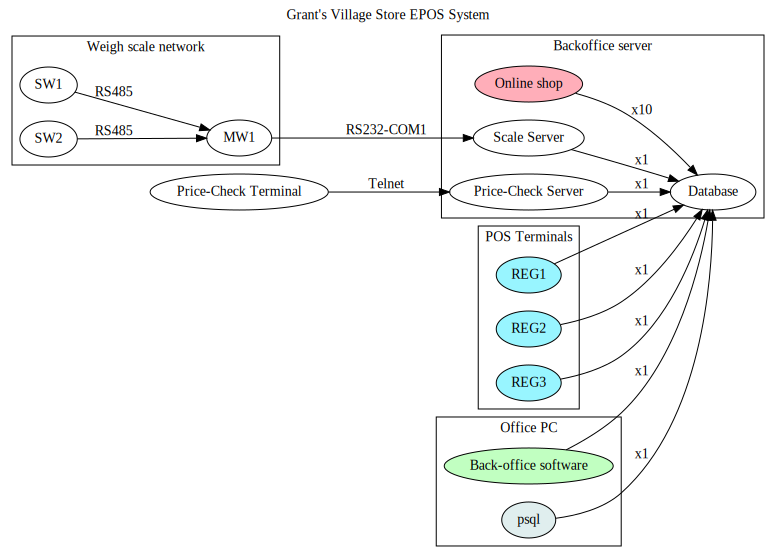
\includegraphics[width=1.0\linewidth]{concurrent_clients}
  \caption{Concurrent clients}
  \label{fig:concurrent-clients}
\end{figure}

\subsubsection{Key points on clients}

\begin{itemize}
\item Clients may be homogeneous (all the same) or heterogenous (different).
\item Some clients may be co-located on one host.
\item Client connection durations may vary:
  \begin{itemize}
  \item Some clients may hold a connection open when idle (desktop or server-side).
  \item Others will open a connection, perform operations and quickly close it.
  \end{itemize}
\item Some clients may maintain a connection pool, where multiple connections are held open and used by individual threads.
\end{itemize}


\section{ACID properties}

\citet{haerder:1983:principles} introduce the so-called ACID properties: \textbf{atomicity}, \textbf{consistency}, \textbf{isolation} and \textbf{durability}.
We will first look at those relevant to a single connection: atomicity, consistency and durability.
Isolation will be treated separately later. Key points to note:
\begin{itemize}
\item Individual ACID characteristics are not orthogonal to each other, and depend on each other in a number of ways.
\item Although we can have a transaction with one or more operations, we assume for the purposes of this section that a transaction has at least two operations. 
\item We say define a transaction as committed once the  \mintinline{postgresql}{COMMIT} SQL statement returns, or the commit method/function of the database connectivity library returns when connecting from application layer code.
\end{itemize}

\subsection{Atomicity}
\label{sec:atomicity}

\citet{haerder:1983:principles} define atomicity of a transaction as:
\begin{quotation}
  It must be of the all-or-nothing type ..., and the user must, whatever happens, know which state he or she is in.
\end{quotation}
(The word atomic also appears when referring to 1NF. This is a separate usage of the term.)

Thus an atomic database transaction is an indivisible or irreducible set of database operations.
Either the transaction succeeds as a single unit or it does not.
Atomicity guarantees that a transaction will not be partially committed.

Consider a basic transaction in a casino backoffice: 
\begin{minted}{postgresql}
-- transfer 20 chips from player 2389 to player 2991
BEGIN; 
UPDATE player SET chips = chips - 20 WHERE id=2389;
UPDATE player SET chips = chips + 20 WHERE id=2991;
COMMIT;
\end{minted}
If the first statement succeeds, issues could subsequently occur:
The second statement may result in errors.
If statements are being issued manually, syntactically correct but commercially erroneous instructions may be issued, and noticed before committing.
The client-server connection itself may be lost during the transaction.
Regardless of the reasons why, the guarantee of atomicity ensures that the transaction is not partially committed unless the COMMIT statement is given.


\subsection{Consistency}
\label{sec:consistency}

Consistency is defined by \citet{haerder:1983:principles} to be:
\begin{quotation}
  A transaction reaching its normal end (EOT, end of transaction), thereby committing its results, preserves the consistency of the database.
  In other words, each successful transaction by definition commits only legal results.
\end{quotation}

In practical terms, this is usually taken to mean that all database constraints (e.g. unique, foreign keys, checks, triggers*) are upheld after the \mintinline{postgresql}{COMMIT} statement returns.

\subsection{Isolation} 
\label{sec:isolation}

Isolation requires that \citep{haerder:1983:principles}:
\begin{quotation}
  Events within a transaction must be hidden from other transactions running concurrently.
\end{quotation}
This means that no other concurrent database connection should see anything about the current transaction until the \mintinline{postgresql}{COMMIT} statement returns.
In practical terms, this is the weakest ACID property.
It is often partially relaxed in the interests of performance, \autoref{sec:transaction-isolation}.

\subsection{Durability} 
\label{sec:durability}

A guarantee of durability requires that \citep{haerder:1983:principles}:
\begin{quotation}
Once a transaction has been completed and has committed its results to the database, the system must guarantee that these results survive any subsequent malfunctions.
\end{quotation}
Generally we assume that the transaction has been stored on disk. 
This characteristic also tells us that once committed, a transaction cannot be rolled back.



\section{Transaction isolation}
\label{sec:transaction-isolation}

In practical terms, isolation is often not perfectly implemented.
The trade-off is a much increased database throughput.

The isolation level determines how strickly transactions are isolated from each other.
To understand the different isolation levels, we must first see what can happen when isolation isn't perfect.

\subsection{Read-phenomena}

A read-phenomenon is said to occur when the data visible to one transaction that has been started does not stay exactly the same until the transaction is finished (committed or rolled back). 
This obviously doesn't include changes made by the transaction itself.

\begin{description}
\item[Phantom read] In the course of a transaction, \textbf{two identical queries} are executed, and the \textbf{collection of rows} returned by the second query is \textbf{different} from the first.
\item[Non-repeatable read] During the course of a transaction, a \textbf{piece of data is retrieved twice} and the \textbf{values differ} between reads.
\item[Dirty read:] A transaction is allowed to \textbf{read data} that has been \textbf{written by another running transaction} and \textbf{not yet committed}.
\item[Serialisation anomaly:] The result of successfully committing a group of transactions is inconsistent with all possible orderings of running those transactions one at a time.
\end{description}
  
\subsection{Isolation levels}

ANSI SQL defines four standard isolation levels.
Each trades increased concurrency against possible read phenomena \autoref{tab:read-phenomena-vs-isolation-level}.

\begin{table}[htbp]
  \centering
  \begin{tabular}{l c c c c}
    \toprule
    \textbf{Isolation level} & \textbf{Dirty read} & \textbf{Non-repeatable read} & \textbf{Phantom read} & \textbf{Serialization anomaly} \\
    \midrule
    Read uncommitted & Y & Y & Y & Y \\
    Read committed & N & Y & Y & Y \\
    Repeatable read & N & N & Y & Y \\
    Serializable & N & N & N & N \\
    \bottomrule
  \end{tabular}
  \caption{Read phenomena possible in each isolation level}
  \label{tab:read-phenomena-vs-isolation-level}
\end{table}

Databases implementing the four isolation levels must guarantee at least the level of isolation specified in the level, that is, none of the prohibited read phenomena must occur.
They can however provide stricter isolation than standards require at any particular level.
See the postgresql manual:\\
https://www.postgresql.org/docs/current/sql-set-transaction.html

Isolation levels are set:
\begin{minted}{postgresql}
-- for transaction 
SET TRANSACTION ISOLATION LEVEL ... ;
-- for transactions in this session
SET SESSION CHARACTERISTICS AS TRANSACTION ISOLATION LEVEL ... ; 
\end{minted}
The explanations below assume PostgreSQL is the database of interest.


\subsubsection{READ UNCOMMITTED}

ANSI standard allows transaction to experience \textbf{dirty reads} of as-yet uncommitted changes made by other transactions.

In practice, PostgreSQL treats this the same as \mintinline{postgresql}{READ COMMITTED}, so dirty reads will never be seen in practice with PostgreSQL.



\subsubsection{READ COMMITTED}

Read Committed guarantees that:
\begin{quotation}
  A statement can only see rows committed before it began. This is the default.
\end{quotation}
Read Committed in essence ensures that the state of the database is consistent with respect to a single command. 
In practice:
\begin{itemize}
\item Protects against dirty reads.
\item \textbf{Phantom reads}, \textbf{Non-repeatable reads} and \textbf{Serialisation anomalies}  possible.
\item Any query is working with the committed state of the database plus any changes made thus far in the current transaction.
\item Some operations may cause the one transaction to have to wait for the other to end (commit or rollback) before they complete.
\end{itemize}

\subsubsection{REPEATABLE READ}

Repeatable Read guarantees that:
\begin{quotation}
  All statements of the current transaction can only see rows committed before the first query or data-modification statement was executed in this transaction.
\end{quotation}
Compared to read committed, it ensures that all statements within a transaction are working with the same consistent view of the database.
In practice:
\begin{itemize}
\item Protects against dirty reads and non-repeatable reads.
\item \textbf{Phantom reads} possible within ANSI standard, but will not occur in PostgreSQL.
\item There may be serialization failures where an update operation cannot proceed because another transaction has committed a change to data that the operation depends on.
\end{itemize}

\subsubsection{SERIALIZABLE}

The PostgreSQL manual defines SERIALIZABLE as:
\begin{quotation}
  The Serializable isolation level provides the strictest transaction isolation. This level emulates serial transaction execution for all committed transactions; as if transactions had been executed one after another, serially, rather than concurrently.
\end{quotation}



